% layout and global options
\documentclass
[
  fontsize = 11pt,
  parskip  = half-,
  BCOR     = 0pt,
  DIV      = 11,
  draft,
  ngerman,
  dvipsnames
]
{scrartcl}

% default packages
\usepackage[utf8]{inputenc}
\usepackage[T1]{fontenc}
\usepackage{babel}
\usepackage{lmodern}
% extra packages
\usepackage{amsmath}
\usepackage{amssymb}
\usepackage{enumerate}
\usepackage{eurosym}
\usepackage{graphicx}
\usepackage{ifthen}
\usepackage{siunitx}
\usepackage{tikz}

% enable calculations in TikZ
\usetikzlibrary{calc}
\usetikzlibrary{decorations.pathreplacing}

% use comma as decimal separator
\sisetup{locale=DE, group-minimum-digits=4}

% no headers no footers
\pagestyle{empty}

% ------------------------------------------------------------------------------
\begin{document}
% ------------------------------------------------------------------------------

\enlargethispage{2\baselineskip}%

% --------------------------------------------------
\section*{Größen und wissenschaftliche Schreibweise}
% --------------------------------------------------
\begin{center}
  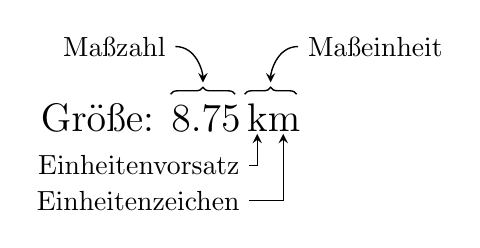
\begin{tikzpicture}
    \node at (0, 0) {\Large Größe: \SI{8.75}{\kilo\metre}};
    \draw[line width=0.5pt, decorate, decoration=brace]
         (0, 2ex)
         -- coordinate (A)
         (8.2mm, 2ex);
    \draw[line width=0.5pt, decorate, decoration=brace]
         (9.4mm, 2ex)
         -- coordinate (B)
         (16mm, 2ex);
    \draw[line width=0.5pt, <-, >=stealth, shorten <=1.5mm]
         (A) to[out=90, in=0] ++(120:7mm)
         node[left] {Maßzahl};
    \draw[line width=0.5pt, <-, >=stealth, shorten <=1.5mm]
         (B) to[out=90, in=180] ++(60:7mm)
         node[right] {Maßeinheit};
    \draw[line width=0.5pt, <-, >=stealth]
         (11mm, -2mm) -- (11mm, -6mm) -- (10mm, -6mm)
         node[left] {Einheitenvorsatz};
    \draw[line width=0.5pt, <-, >=stealth]
         (14.3mm, -2mm) -- (14.3mm, -10.5mm) -- (10mm, -10.5mm)
         node[left] {Einheitenzeichen};
  \end{tikzpicture}
\end{center}

% -----------------------------
\subsection*{Einheitenvorsätze}
% -----------------------------
\begin{center}
  \renewcommand{\arraystretch}{1.1}%
  \begin{tabular}{|r|l|c|l|}
    \hline
    \textbf{Vorsatz}  &
    \textbf{Name}     &
    \textbf{Potenz}   &
    \textbf{Zahlwort} \\
    \hline
    Y       & Yotta & $10^{24}$  & Quadrillion     \\
    Z       & Zetta & $10^{21}$  & Trilliarde      \\
    E       & Exa   & $10^{18}$  & Trillion        \\
    P       & Peta  & $10^{15}$  & Billiarde       \\
    T       & Tera  & $10^{12}$  & Billion         \\
    G       & Giga  & $10^{9}$   & Milliarde       \\
    M       & Mega  & $10^{6}$   & Million         \\
    k       & Kilo  & $10^{3}$   & Tausend         \\
    h       & Hekto & $10^{2}$   & Hundert         \\
    da      & Deka  & $10^{1}$   & Zehn            \\
    \hline
    d       & Dezi  & $10^{-1}$  & Zehntel         \\
    c       & Zenti & $10^{-2}$  & Hundertstel     \\
    m       & Milli & $10^{-3}$  & Tausendstel     \\
    $\mu$   & Mikro & $10^{-6}$  & Millionstel     \\
    n       & Nano  & $10^{-9}$  & Milliardstel    \\
    p       & Piko  & $10^{-12}$ & Billionstel     \\
    f       & Femto & $10^{-15}$ & Billiardstel    \\
    a       & Atto  & $10^{-18}$ & Trillionstel    \\
    z       & Zepto & $10^{-21}$ & Trilliardstel   \\
    y       & Yokto & $10^{-24}$ & Quadrillionstel \\
    \hline
  \end{tabular}%
\end{center}

% -------------------------------------
\subsection*{Physikalische Basisgrößen}
% -------------------------------------
\begin{center}
  \begingroup
    %\setlength{\tabcolsep}{1em}%
    \renewcommand{\arraystretch}{1.1}%
    \begin{tabular}{|l|l|c|}
      \hline
      \textbf{Dimension}        &
      \textbf{Einheit}          &
      \textbf{Einheitenzeichen} \\
      \hline
      Zeit        & Sekunde & s   \\
      \hline
      Länge       & Meter   & m   \\
      \hline
      Masse       & Gramm   & g   \\
      \hline
      Temperatur  & Kelvin  & K   \\
      \hline
      Stromstärke & Ampere  & A   \\
      \hline
      Lichtstärke & Candela & cd  \\
      \hline
      Stoffmenge  & Mol     & mol \\
      \hline
    \end{tabular}
  \endgroup
\end{center}

% ------------------------------------------------------------------------------
\end{document}
% ------------------------------------------------------------------------------

